The tasks required in the 2016 UAV Challenge are such that a purely fixed-wing or rotor-based aircraft is unlikely to be successful; instead, teams will need to design an aircraft that makes use of both flight modes. Analysis of the 2014 design, a purely fixed-wing aircraft, showed that converting it to a hybrid aircraft would not result in a suitable design for the Challenge. Given the aircraft's weight, adding the necessary equipment would add over 5kg, cost over \$500, and would result in less than 60 seconds of flight time. It was therefore decided the 2014 model would not be suitable for the 2016 competition; a detailed analysis can be found in Appendix \ref{sec:lastYear}.\\

As this project involves the development of a novel aircraft platform, there is a lack of academic literature that is relevant to the problem at hand. This review will instead collate examples of commercial and hobby systems that were used to inspire and guide the development of the aircraft.\\

\subsection{Aircraft Design}
\subsubsection*{Arcturus Jump}
The Arcturus Jump\cite{ref:arcturus} (Figure \ref{fig:arcturus}) is a quad-copter/fixed-wing hybrid, with propellers mounted across the wings for VTOL, and a propeller at the front for fixed-wing flight. Modifying an existing airframe to emulate this design would be straightforward, but the addition of the support structure for VTOL flight would add significant weight to the aircraft, decreasing thrust and maneuverability, and increasing drag. These factors make an aircraft of this design unlikely to achieve \textbf{R4} (60km endurance) and \textbf{R5} (60min of flight) of the UAV Challenge.

\begin{figure}[!h]
	\centering
	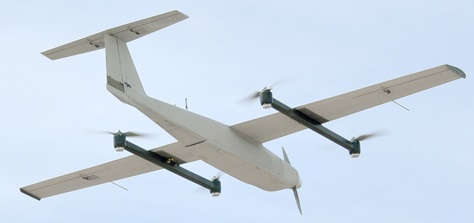
\includegraphics[width=150pt]{\IMAGEPATH /Aircraft/arcturus}
	\caption{Arcturus Jump 20}
	\label{fig:arcturus}
\end{figure}

\subsubsection*{X PlusOne}
The X PlusOne\cite{ref:xplusone} (Figure \ref{fig:xplusone}) is an incredibly fast and efficient hybrid with four front-facing propellers. It is extremely small and light, and would be relatively cheap to build, but is too small to replicate with an existing airframe. Designing a new airframe would take a significant amount of time, and is outside the scope of the project.
\todomessage{Change "outside of scope"}

\begin{figure}[!ht]
	\centering
	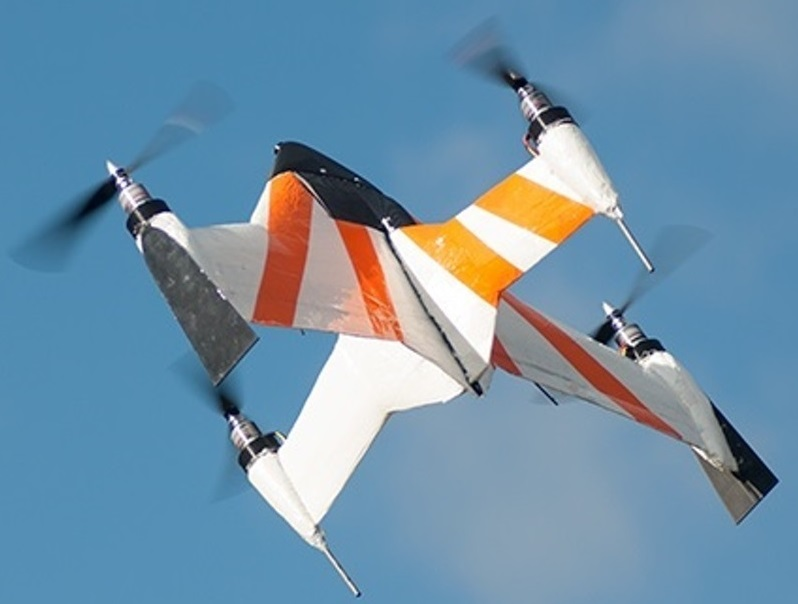
\includegraphics[width=120pt]{\IMAGEPATH /Aircraft/xplusone}
	\caption{X PlusOne}
	\label{fig:xplusone}
\end{figure}

\subsubsection*{TBS Caipirinha}
The TBS Caipirinha\cite{ref:caipirinha} (Figure \ref{fig:caipirinha}) is traditionally a hobbyist fixed-wing aircraft kit. However, several examples have shown it is possible to modify the Caipirinha to be a VTOL aircraft\cite{ref:caipirinhaVTOL} (Figure \ref{fig:caipirinhaVTOL}), with two front-facing propellers. Modifying the Caipirinha for hybrid flight would require minimal modifications to the airframe but would require the development of advanced control systems to alternate between VTOL and fixed-wing modes, which outside the scope of this project.
\todomessage{Change "outside of scope"}

\begin{figure}[!ht]
	\centering
	\begin{minipage}{.5\textwidth}
		\centering
		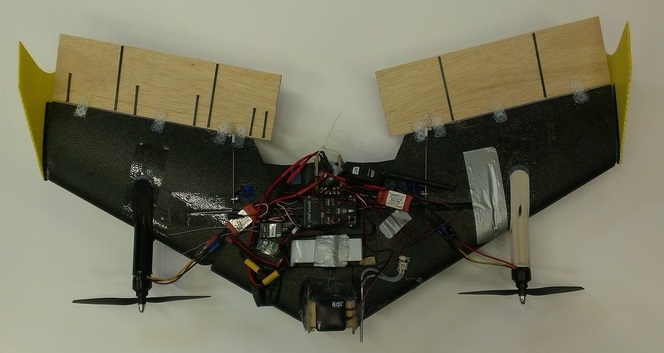
\includegraphics[width=135pt]{\IMAGEPATH /Aircraft/caipirinha}
		\caption{TBS Caipirinha}
		\label{fig:caipirinha}
	\end{minipage}%
	\begin{minipage}{.5\textwidth}
		\centering
		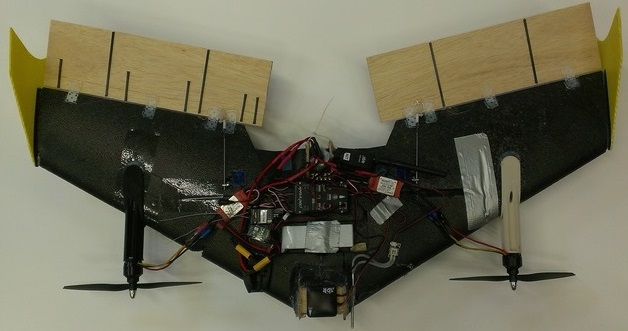
\includegraphics[width=155pt]{\IMAGEPATH /Aircraft/caipirinhaVTOL}
		\caption{Caipirinha modified for VTOL flight}
		\label{fig:caipirinhaVTOL}
	\end{minipage}
\end{figure}

\subsubsection*{Aerosense AS-DT01-E}
The Aerosense AS-DT01-E\cite{ref:sony} (Figure \ref{fig:sony}) is an autonomous hybrid VTOL/fixed-wing aircraft being developed by Sony Mobile in partnership with Japanese company ZMP. While the prototype aircraft would be an ideal candidate for the Challenge, as with the X PlusOne the design and construction of the airframe would be time consuming, and is outside the scope of this project.
\todomessage{Change "outside of scope"}

\begin{figure}[!ht]
	\centering
	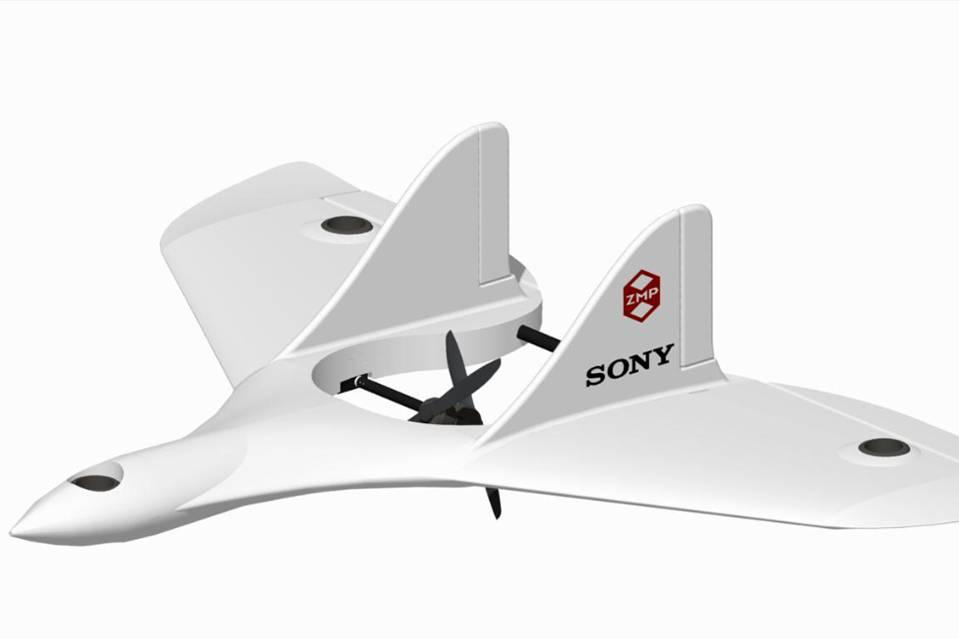
\includegraphics[width=160pt]{\IMAGEPATH /Aircraft/sony}
	\caption{Sony Aerosense}
	\label{fig:sony}
\end{figure}

\subsubsection*{FireFLY6}
Finally, the FireFLY6\cite{ref:firefly6} (Figure \ref{fig:firefly6}) is a remote control hybrid VTOL/fixed-wing aircraft consisting of six propellers arranged in 3 sets of two (Y6 configuration). This design can achieve 20-30 minutes of flight time, seven minutes of hover, and a cruising speed of 54km/h, and would be a strong contender in the UAV Challenge.

\begin{figure}[!h]
	\centering
	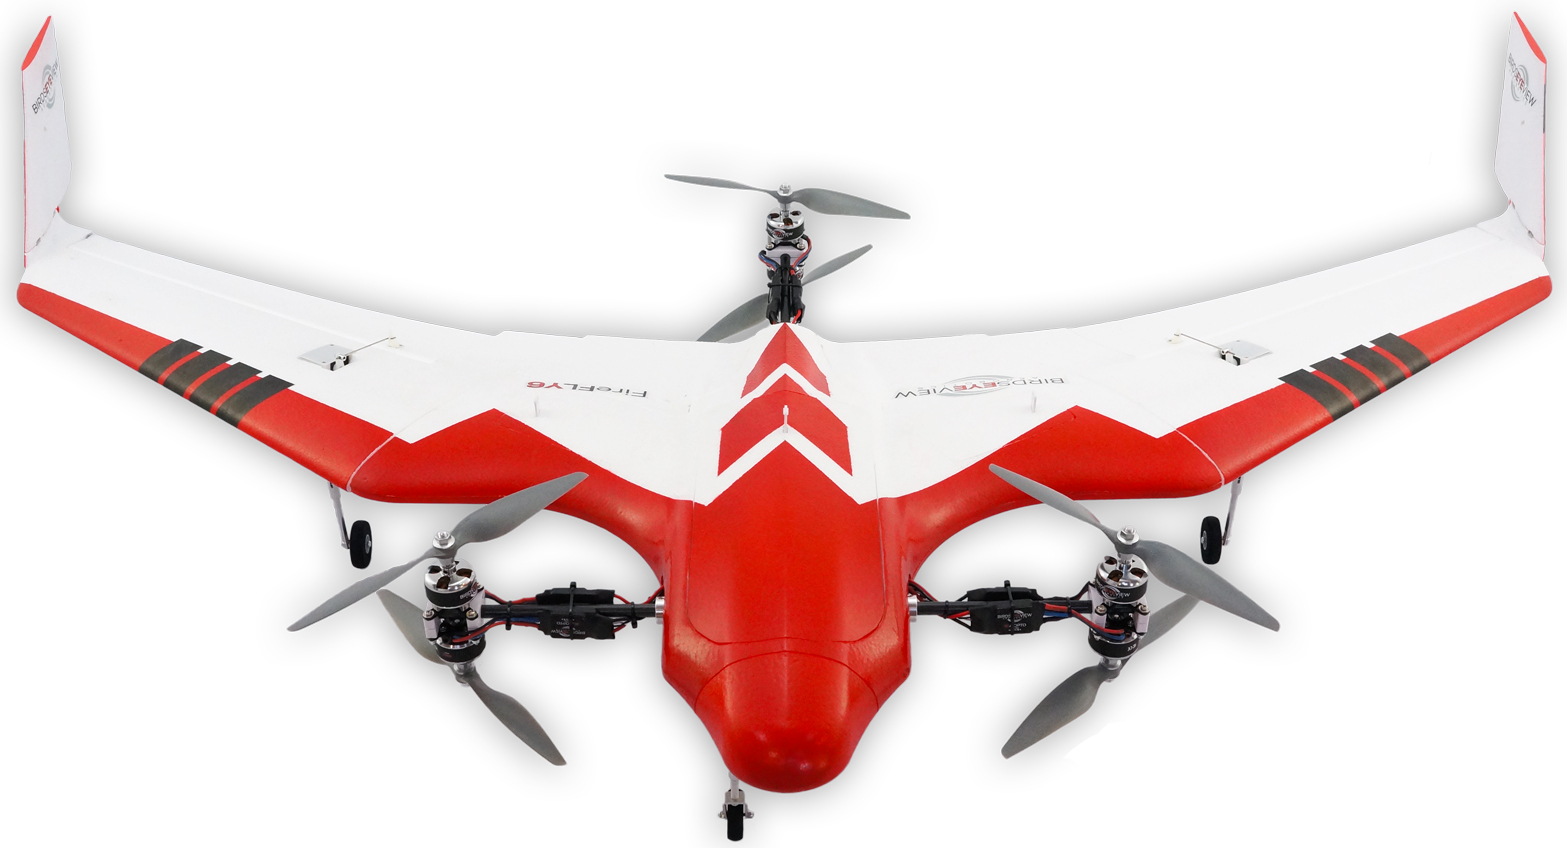
\includegraphics[width=160pt]{\IMAGEPATH /Aircraft/firefly6}
	\caption{FireFLY6}
	\label{fig:firefly6}
\end{figure}

\subsection{Flight Systems}
\subsubsection*{Flight Control}
The addition of a flight controller to the aircraft permits autonomous flight capabilities, including way point planning and motor control. The most viable (and well supported) options are the PixHawk\cite{ref:pixhawk}, APM 2.6\cite{ref:ardupilot}, and PX4\cite{ref:px4}. In order to achieve reliable and safe autonomous flight the controller must be fast and have sufficient storage for additional firmware/software to extend its capabilities. A comparison of each option may be found in \cite{ref:controller_comparison}, showing that given its larger memory storage, faster processor, and additional capabilities such as in-built gyroscopes and accelerometers, the PixHawk is the best choice for this project.

\subsubsection*{Controller Development}
The PixHawk flight controller has several flight control systems readily available for many types of aircraft (including fixed-wing and VTOL), but as of yet has no control system designed for a hybrid aircraft. Fortunately, the PX4 firmware (on which the PixHawk is based) is Open Source\cite{ref:ardupilotgit}, with several resources available\cite{ref:firmware1,ref:firmware2} to allow hobbyists and developers to customize the behaviour of their aircraft.

\subsection{Proposed Design}
Given the aircraft designs presented above, the most suitable option for this project is the FireFLY6. The FireFLY6's motor configuration can be easily replicated using a Skywalker X8. In addition, the X8 is purpose designed to mount various sensors (such as a camera) to its frame.\\

The initial design for this project will use a PixHawk flight controller in a Skywalker X8 airframe, mounted with six motors in Y6 configuration, as with the FireFLY6. The aircraft will also be fitted with a transition system, to rotate the front motors and enable the aircraft to fly in both VTOL and fixed-wing modes. Finally, the aircraft will be mounted with various sensors, including a camera and LiDAR, to provide sensing capabilities for planning, obstacle detection and autonomous flight.